\documentclass{article}
\input{../preamble}
\geometry{margin=1in}
\setlength{\parskip}{1em}
\pgfplotsset{compat=1.9, width=220pt}

\begin{document}

Physics \hfill Worksheet \thepage \hfill Date

\textbf{For each of the velocity vs.~time graphs below, calculate the displacement (\textit{i.e.}, the net change in position, $\Delta x$). The first plot has been completed as an example.}

\fbox{\fbox{%
  \parbox{0.97\textwidth}{

\begin{tikzpicture}
\begin{axis}[color=black,axis y line=left, 
    axis x line=left,
    ymin=0, ymax=125,
    xmin=0, xmax=30,
    ylabel = Velocity (m/s),
    xlabel = Time (s),
    grid=both,
    ytick={0,25,...,175}
]
\addplot[name path=f,domain=0:30,ultra thick,black
] 
coordinates{
    (0,0)
    (20,100)
    (30,100)
};
\end{axis}
\end{tikzpicture}%
\hfill
\begin{tikzpicture}
\begin{axis}[color=black,axis y line=left, 
    axis x line=left,
    ymin=0, ymax=125,
    xmin=0, xmax=30,
    ylabel = Velocity (m/s),
    xlabel = Time (s),
    ytick={0,25,...,175},
    clip=false,
]

\filldraw[black!15!] 
    (axis cs: 0,0.5) -- 
    (axis cs: 30,0.5) -- 
    (axis cs: 30,100) -- 
    (axis cs: 20,100);

\addplot[domain=0:30,ultra thick,black
    ] 
    coordinates {
    (0,0)
    (20,100)
    (30,100)
    };
    
\addplot[
    %color=green!67!black,
    color=black,
    mark options={color=black},mark=none,
    ultra thick,dashed,
    ]
    coordinates {
    (20,0)(20,100)
    };
\node[red] at (axis cs: 9,95){%
  $\begin{aligned}
     A_1 &= \frac{1}{2} b h\\
         &= \frac{1}{2} \left(20\right) \left(100\right)\\
         &= 1000\\
  \end{aligned}$};
\draw[->,red,thick] (axis cs: 9,67) --++ (axis cs: 3,-27);
%\node (axis cs:25,50) {\large $A_2 = b h $};

\node[red] at (axis cs: 25,123){%
  $\begin{aligned}
     A_2 &= b h\\
         &= \left(10\right) \left(100\right)\\
         &= 1000\\
  \end{aligned}$};

\draw[->, red, thick] (axis cs: 25,105) --++ (axis cs: 0,-20) ;


\filldraw[white] 
    (axis cs: 7,10) --
    (axis cs: 29,10) --
    (axis cs: 29,30) --
    (axis cs: 7,30);
\draw  (axis cs: 7,10) --
    (axis cs: 29,10) --
    (axis cs: 29,30) --
    (axis cs: 7,30) --
    (axis cs: 7,10);
\node[red,anchor=west] at (axis cs: 8,20) {$ \Delta x = A_1 + A_2 = \SI{2000}{m}$};
\end{axis}
\end{tikzpicture}
}}}

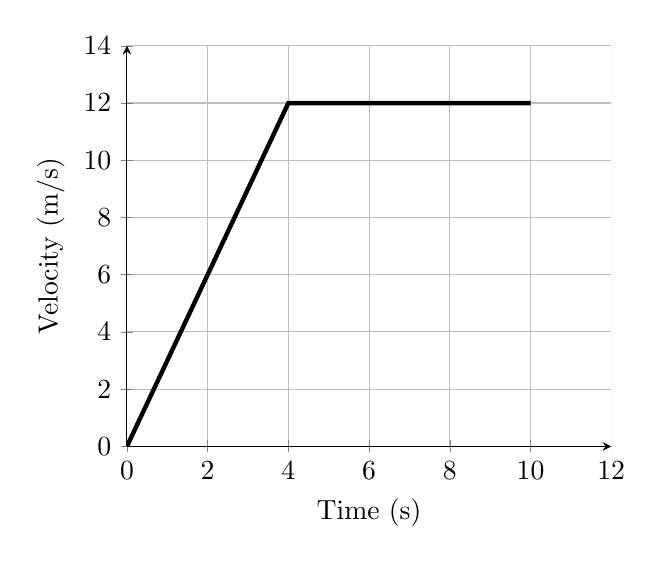
\begin{tikzpicture}
    \begin{axis}[axis y line=left, 
        axis x line=left,
        ymin=0, ymax=14,
        xmin=0, xmax=12,
        ylabel = Velocity (m/s),
        xlabel = Time (s),
        grid=both,
        ytick={0,2,...,14}
    ]
    \addplot[
        %color=green!67!black,
        color=black,
        mark options={color=black},mark=none,
        ultra thick,
        ]
        coordinates {
        (0,0)
        (4,12)
        (10,12)
        };
    \end{axis}
\end{tikzpicture}%
\hfill
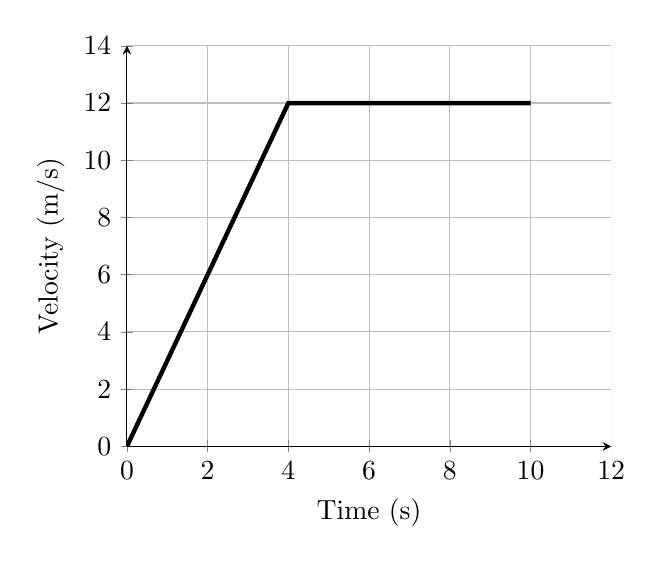
\begin{tikzpicture}
    \begin{axis}[axis y line=left, 
        axis x line=left,
        ymin=0, ymax=14,
        xmin=0, xmax=12,
        ylabel = Velocity (m/s),
        xlabel = Time (s),
        grid=both,
        ytick={0,2,...,14}
    ]
    \addplot[
        %color=green!67!black,
        color=black,
        mark options={color=black},mark=none,
        ultra thick,
        ]
        coordinates {
        (0,0)
        (4,12)
        (10,12)
        };
    \end{axis}
\end{tikzpicture}

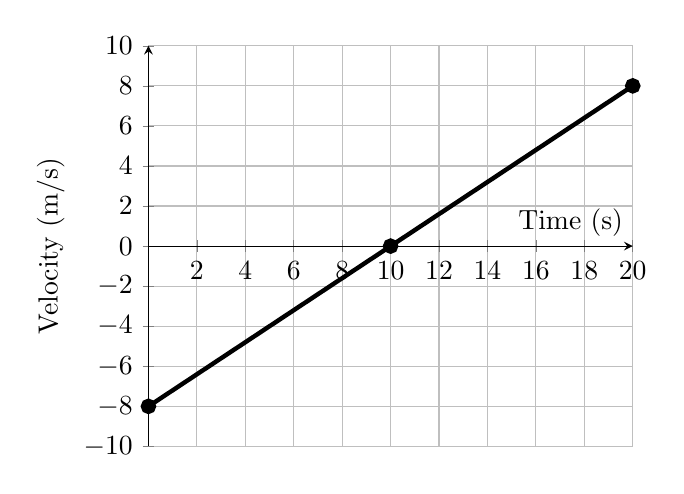
\begin{tikzpicture}
\begin{axis}[
    axis y line=left, 
    axis x line=center,
    xlabel = Time (s),
    ylabel = Velocity (m/s),
    ymin=-10, ymax=10,
    xmin=0, xmax=20,
    ytick={-10,-8,...,10},
    xtick={0,2,...,20},
    ymajorgrids=true,
    xmajorgrids=true,
    % x label style={anchor=west},
    clip=false,
]
    \addplot[
        %color=green!67!black,
        color=black,
        mark options={color=black},mark=*,
        ultra thick,
        ]
        coordinates {
        (0,-8)
        (10,0)
        (20,8)
        };
\end{axis}
\end{tikzpicture}%
\hfill
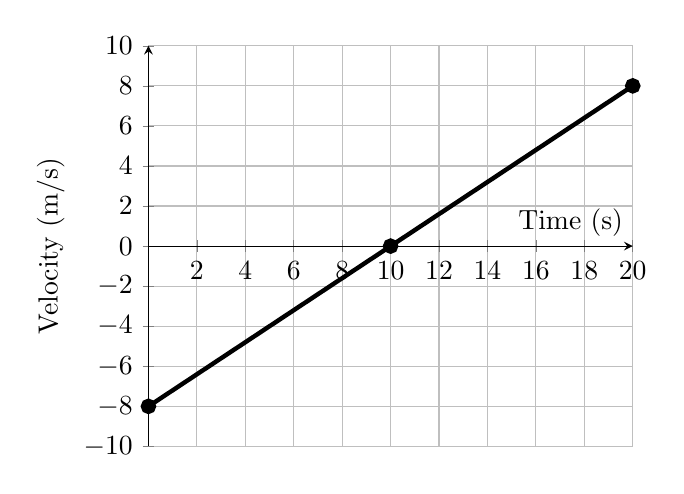
\begin{tikzpicture}
\begin{axis}[
    axis y line=left, 
    axis x line=center,
    xlabel = Time (s),
    ylabel = Velocity (m/s),
    ymin=-10, ymax=10,
    xmin=0, xmax=20,
    ytick={-10,-8,...,10},
    xtick={0,2,...,20},
    ymajorgrids=true,
    xmajorgrids=true,
    % x label style={anchor=west},
    clip=false,
]
    \addplot[
        %color=green!67!black,
        color=black,
        mark options={color=black},mark=*,
        ultra thick,
        ]
        coordinates {
        (0,-8)
        (10,0)
        (20,8)
        };
\end{axis}
\end{tikzpicture}

\end{document}